\documentclass{sigchi-ext}
% Please be sure that you have the dependencies (i.e., additional
% LaTeX packages) to compile this example.
\usepackage[T1]{fontenc}
\usepackage{textcomp}
\usepackage[scaled=.92]{helvet} % for proper fonts
\usepackage{graphicx} % for EPS use the graphics package instead
\usepackage{balance}  % for useful for balancing the last columns
\usepackage{booktabs} % for pretty table rules
\usepackage{ccicons}  % for Creative Commons citation icons
\usepackage{ragged2e} % for tighter hyphenation

% \usepackage{marginnote} \usepackage[shortlabels]{enumitem}
% \usepackage{paralist}

%% EXAMPLE BEGIN -- HOW TO OVERRIDE THE DEFAULT COPYRIGHT STRIP --
% \copyrightinfo{Permission to make digital or hard copies of all or
% part of this work for personal or classroom use is granted without
% fee provided that copies are not made or distributed for profit or
% commercial advantage and that copies bear this notice and the full
% citation on the first page. Copyrights for components of this work
% owned by others than ACM must be honored. Abstracting with credit is
% permitted. To copy otherwise, or republish, to post on servers or to
% redistribute to lists, requires prior specific permission and/or a
% fee. Request permissions from permissions@acm.org.\\
% {\emph{CHI'14}}, April 26--May 1, 2014, Toronto, Canada. \\
% Copyright \copyright~2014 ACM ISBN/14/04...\$15.00. \\
% DOI string from ACM form confirmation}
%% EXAMPLE END

\title{Wikidata Human Gender Index}

\numberofauthors{4}
% Notice how author names are alternately typesetted to appear ordered
% in 2-column format; i.e., the first 4 autors on the first column and
% the other 4 auhors on the second column. Actually, it's up to you to
% strictly adhere to this author notation.
\author{%
  \alignauthor{%
    \textbf{First Author}\\
    \affaddr{University of Author} \\
    \affaddr{Authortown, CA 94022, USA} \\
    \affaddr{author1@anotherco.edu} }\alignauthor{%
    \textbf{Fifth Author}\\
    \affaddr{YetAuthorCo, Inc.}\\
    \affaddr{Authortown, BC V6M 22P Canada}\\
    \email{author5@anotherco.com} } \vfil \alignauthor{%
    \textbf{Second Author}\\
    \affaddr{VP, Authoring}\\
    \affaddr{Authorship Holdings, Ltd.}\\
    \affaddr{Awdur SA22 8PP, UK}\\
    \email{author2@author.ac.uk} }\alignauthor{%
    \textbf{Sixth Author}\\
    \affaddr{Universit\'e de Auteur-Sud}\\
    \affaddr{40222 Auteur France}\\
    \email{author6@author.fr} } \vfil \alignauthor{%
    }
    }	

% Paper metadata (use plain text, for PDF inclusion and later
% re-using, if desired)
\def\plaintitle{SIGCHI Extended Abstracts Sample File: Note Initial
  Caps} \def\plainauthor{First Author, Second Author, Third Author,
  Fourth Author, Fifth Author, Sixth Author}
\def\plainkeywords{Authors' choice; of terms; separated; by
  semicolons; include commas, within terms only; required.}
\def\plaingeneralterms{Documentation, Standardization}

%% Set up our PDF with metadata
\hypersetup{%
  pdftitle={\plaintitle}, pdfauthor={\plainauthor},
  pdfkeywords={\plainkeywords}, }

% \reversemarginpar%

\begin{document}

\maketitle

% Uncomment to disable hyphenation (not recommended)
% https://twitter.com/anjirokhan/status/546046683331973120
\RaggedRight{} 

% Do not change the page size or page settings.
\begin{abstract}
  UPDATED---\today. This sample paper describes the formatting
  requirements for SIGCHI Extended Abstract Format, and this sample
  file offers recommendations on writing for the worldwide SIGCHI
  readership. Please review this document even if you have submitted
  to SIGCHI conferences before, as some format details have changed
  relative to previous years. Abstracts should be about 150
  words. Required.
\end{abstract}

\keywords{\plainkeywords}

\category{H.5.m}{Information interfaces and presentation (e.g.,
  HCI)}{Miscellaneous}\category{See}{\url{http://acm.org/about/class/1998/}}{for
  full list of ACM classifiers. This section is required.}

\section{Introduction}
Problematize introduction and make obvious need.

Landscape of ways in which Wikipedia shows bias, and Landscape of biases.

Our first observation is from September 17th 2014, and latest is January 3rd 2016. Although our dataset is now updated weekly following the official data dumps, automation was not completed until June 28th 2015, and so there is a window missing from October 2014 to June 2015. 
\section{Description}

The Data is collected by (I'm sure I've written this somewhere already).

Total human in wikidata increased from $5,869,606$ to $6,999,542$.
\begin{figure}
\label{totalhumans}
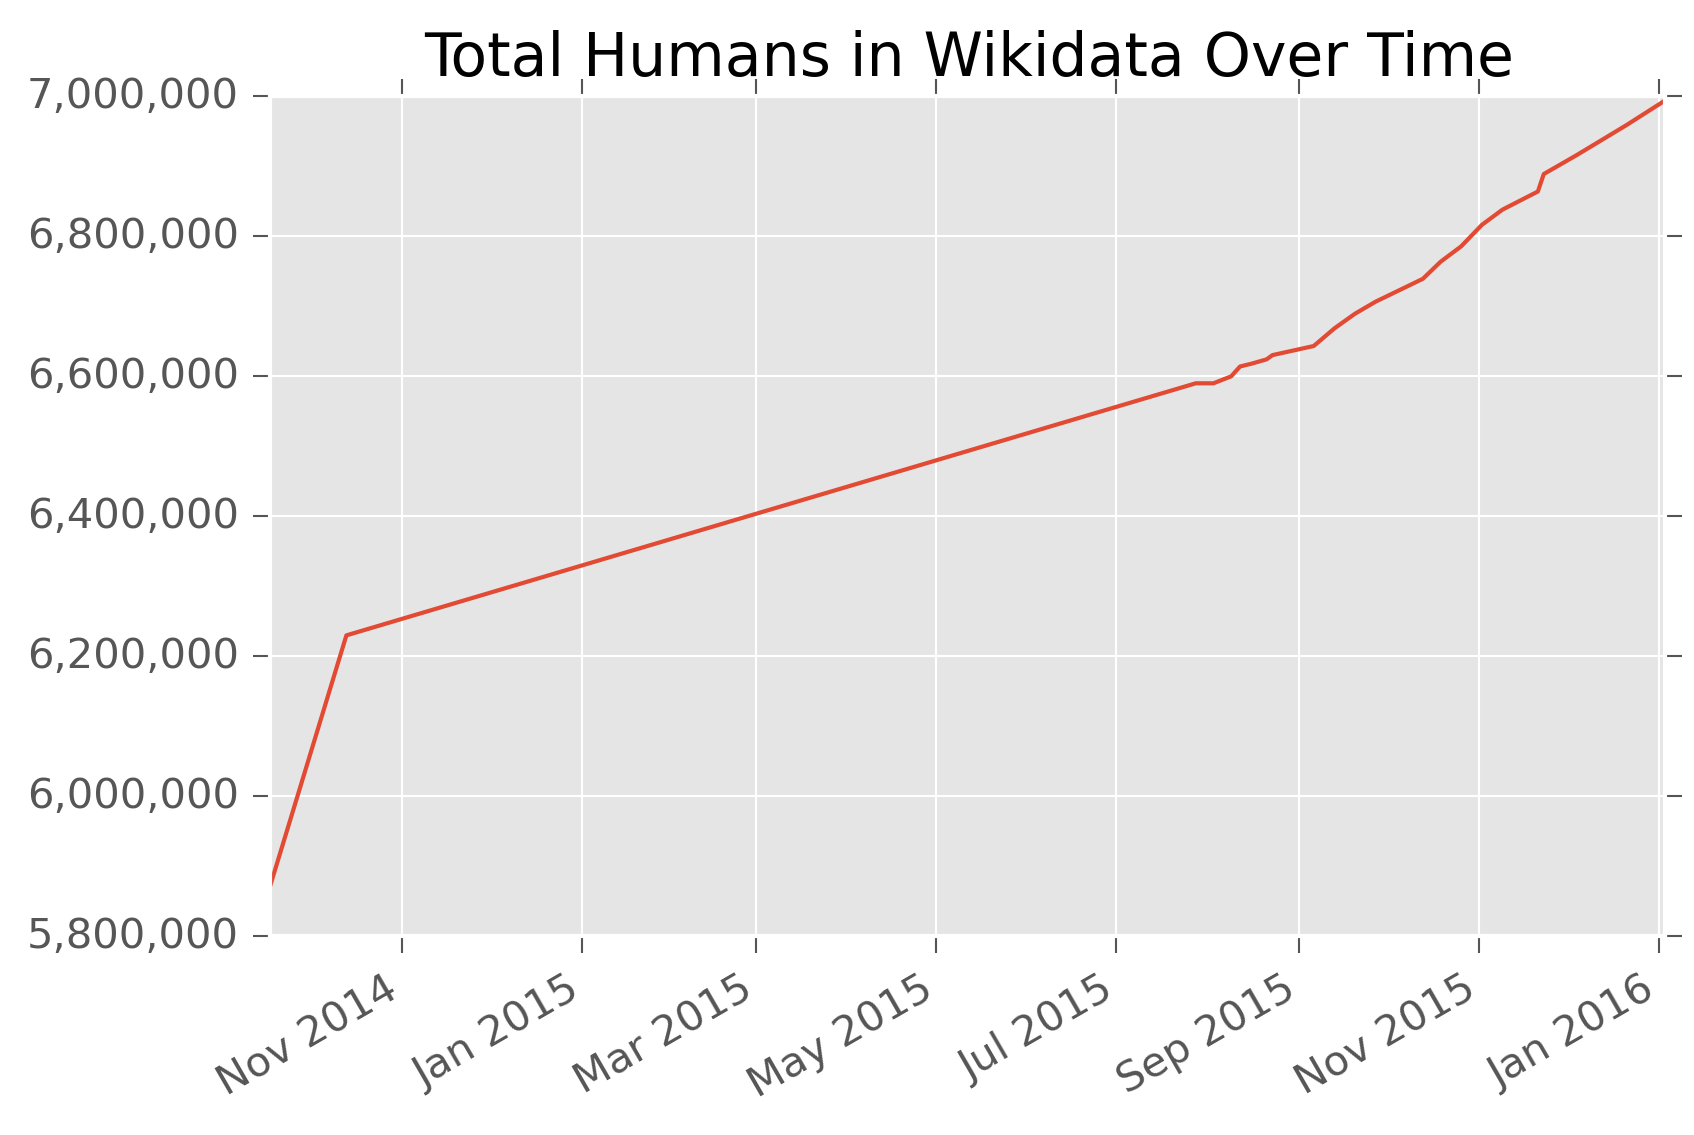
\includegraphics[scale=0.6]{figures/totalhumans.png} 
\caption{Total number of humans found in Wikidata at each snapshot period.}
\end{figure}

We should also be curious to the data quality of the increasing humans. One way to think about this is about the how much data is accompanying these human entries. 

\begin{table}
\begin{tabular}{lrrrrr}
\toprule
{} &  citizenship &  place of birth &  ethnic group &  at least 1 site link &    gender \\
\midrule
2014-09-17 &     0.428217 &        0.240124 &      0.003109 &              0.996164 &  0.952879 \\
2016-01-03 &     0.582185 &        0.305102 &      0.005559 &              0.981463 &  0.965416 \\
\bottomrule
\end{tabular}
\label{table:accompanying}
\caption{Accompanying properties at }
\end{table}





\subsection{Descriptive Statistics}



% \bibliographystyle{ACM-Reference-Format-Journals}
\bibliographystyle{SIGCHI-Reference-Format}
% \bibliographystyle{acm}
\bibliography{sample}

\end{document}

%%% Local Variables:
%%% mode: latex
%%% TeX-master: t
%%% End:
